\documentclass[12pt,a4paper]{report}
\usepackage[utf8]{inputenc}
\usepackage{graphicx}
\usepackage{geometry}
\usepackage{setspace}
\usepackage{titlesec}
\usepackage{tabularx}
\usepackage{booktabs}
\usepackage{hyperref}
\usepackage{amsmath}
\usepackage{listings}
\usepackage{xcolor}

\geometry{top=1.0in, bottom=0.8in, left=1.0in, right=0.8in}
\setstretch{1.35}

\definecolor{codegreen}{rgb}{0,0.6,0}
\definecolor{codegray}{rgb}{0.5,0.5,0.5}
\definecolor{codepurple}{rgb}{0.58,0,0.82}
\definecolor{backcolour}{rgb}{0.96,0.96,0.96}

\lstdefinestyle{mystyle}{
    backgroundcolor=\color{backcolour},   
    commentstyle=\color{codegreen},
    keywordstyle=\color{magenta},
    numberstyle=\tiny\color{codegray},
    stringstyle=\color{codepurple},
    basicstyle=\ttfamily\footnotesize,
    breakatwhitespace=false,         
    breaklines=true,                 
    captionpos=b,                    
    keepspaces=true,                 
    numbers=left,                    
    numbersep=5pt,                  
    showspaces=false,                
    showstringspaces=false,
    showtabs=false,                  
    tabsize=2
}
\lstset{style=mystyle}

\begin{document}

% ================= COVER PAGE =================
\begin{titlepage}
\centering
\vspace*{0.2cm}
\begin{figure}[h!]
\centering

\includegraphics[width=1.5in]{report_assets/image1.jpeg} \hspace{0.5in}

\includegraphics[width=2.4in]{report_assets/image2.jpeg}
\end{figure}

\vspace{0.8cm}
{\Large \textbf{FINAI WALLET ANALYZER}\par}
\vspace{0.3cm}
{\normalsize \textbf{AI-Assisted Digital Wallet Transaction Analyzer, Auto-Segregator, and Month-End Spend Forecaster}\par}

\vspace{1.2cm}
{\large \textbf{A MINI PROJECT REPORT}\par}
\vspace{0.4cm}
{\normalsize Submitted by\par}
\vspace{0.3cm}
\textbf{KIRTHIKA R \quad (713524CS067)}\\
\textbf{MADANIKA S \quad (713524CS075)}\\
\textbf{MAHANASRI M \quad (713524CS077)}\\
\textbf{MUKILA N \quad (713524CS088)}\\

\vspace{1.2cm}
{\normalsize in partial fulfillment for the award of the degree of\par}
\vspace{0.2cm}
{\large \textbf{BACHELOR OF ENGINEERING}\par}
\vspace{0.2cm}
{\normalsize in\par}
\vspace{0.2cm}
{\large \textbf{COMPUTER SCIENCE AND ENGINEERING}\par}
\vspace{0.4cm}
{\textbf{SNS COLLEGE OF TECHNOLOGY, COIMBATORE 641035}\par}
\vspace{0.4cm}
{\textbf{November 2026}\par}
\end{titlepage}

% ================= BONAFIDE CERTIFICATE =================
\newpage
\begin{center}

\includegraphics[width=1.2in]{report_assets/image1.jpeg} \hspace{0.3in}

\includegraphics[width=2.0in]{report_assets/image2.jpeg}

\vspace{0.5cm}
{\large \textbf{SNS COLLEGE OF TECHNOLOGY, COIMBATORE 641035}\par}
\vspace{0.3cm}
{\Large \textbf{BONAFIDE CERTIFICATE}\par}
\end{center}

\vspace{0.6cm}
Certified that this mini Project Report titled, ``\textbf{FINAI WALLET ANALYZER - AI-Assisted Digital Wallet Transaction Analyzer, Auto-Segregator, and Month-End Spend Forecaster}'' is the bonafide record of ``\textbf{Kirthika R (713524CS067), Madanika S (713524CS075), Mahanasri M (713524CS077), Mukila N (713524CS088)}'' who carried out the mini Project Work under our supervision. Certified further, that to the best of my knowledge the work reported herein does not form part of any other mini project report or dissertation on the basis of which a degree or award was conferred on an earlier occasion on this or any other candidate.

\vspace{2.5cm}
\noindent
\textbf{PROJECT GUIDE} \hfill \textbf{HEAD OF THE DEPARTMENT}\\
\textbf{Ms. V. Vaishnavee} \hfill \textbf{Dr. M. Shobana}\\
Assistant Professor, AI \& DS \hfill Associate Professor \& Head, CSE\\
SNS College of Technology \hfill SNS College of Technology\\
Coimbatore - 641035. \hfill Coimbatore - 641035.\\

\vspace{1.5cm}
\noindent
Submitted for the Viva-Voce examination held at SNS COLLEGE OF TECHNOLOGY, on \dotfill

\vspace{1.5cm}
\noindent
\textbf{Examiner 1} \hfill \textbf{Examiner 2}

% ================= ABSTRACT =================
\newpage
\begin{center}
{\Large \textbf{ABSTRACT}\par}
\end{center}
\vspace{0.5cm}
Digital wallet applications have made peer-to-peer and merchant payments fast and ubiquitous. However, standard wallet applications restrict their utility to transactional logs without offering meaningful financial insights. Users often find it difficult to analyze their spending habits across fragmented apps (such as Google Pay, PhonePe, Paytm, Amazon Pay, and Apple Pay), adhere to categorical budgets, forecast month-end liquidity, or detect suspicious transactions. The FinAI Wallet Analyzer resolves this problem by implementing an intelligent financial management platform utilizing Natural Language Processing (NLP), rule-based anomaly detection, and voice conversational interfaces.

FinAI automatically categorizes transactions into eight distinct classes, assigns necessity tiers (Need vs. Want), and audits fraudulent activities using a multi-parameter risk evaluation scoring matrix. A predictive month-end spend forecaster calculates burn velocity, dynamic safe daily spend allowances, and month-end trajectory curves. In addition, an AI Voice Assistant captures spoken voice commands, extracts financial entities, and confirms transactions hands-free. Built using React 18, Vite, Tailwind CSS, Python FastAPI, SQLite, and a zero-server clientEngine.js localStorage fallback, the system delivers high performance, offline resiliency, and privacy-first personal financial telemetry.

% ================= TABLE OF CONTENTS =================
\newpage
\tableofcontents

\newpage
\chapter{Introduction}
\section{Background}
Over the past decade, rapid digitization and the proliferation of smartphone applications have revolutionized the financial ecosystem. Unified Payments Interface (UPI) and digital wallets process tens of billions of transactions monthly. However, current wallet apps remain predominantly transactional passbooks rather than intelligent financial advisors. Users execute transactions across multiple platforms without an aggregate view of their expenditures.

\section{Project Overview}
FinAI Wallet Analyzer is an intelligent financial management system designed to provide deep telemetry over digital transactions. Driven by NLP heuristics, statistical forecasting, and Web Speech technology, it unifies fragmented wallets, categorizes spending, audits transaction risks, and projects budgetary runways.

\section{Motivation}
Modern consumers suffer from fiscal opacity due to zero payment friction coupled with high accounting friction. Manual expense recording in spreadsheets is unsustainable. FinAI automates categorization, detects anomalies, and informs users in plain language what they can safely spend each day.

\section{Objectives}
\begin{itemize}
    \item Provide unified multi-wallet transaction aggregation and analytics.
    \item Autonomously categorize expenditures using keyword NLP heuristics.
    \item Execute real-time anomaly and fraud risk scoring (Low, Medium, High).
    \item Calculate dynamic safe daily spend quotas and month-end trajectories.
    \item Provide an interactive hands-free Voice Assistant for payment entry and balance queries.
    \item Enable resilient dual-mode operation via an offline clientEngine.js storage layer.
\end{itemize}

\begin{figure}[h!]
\centering
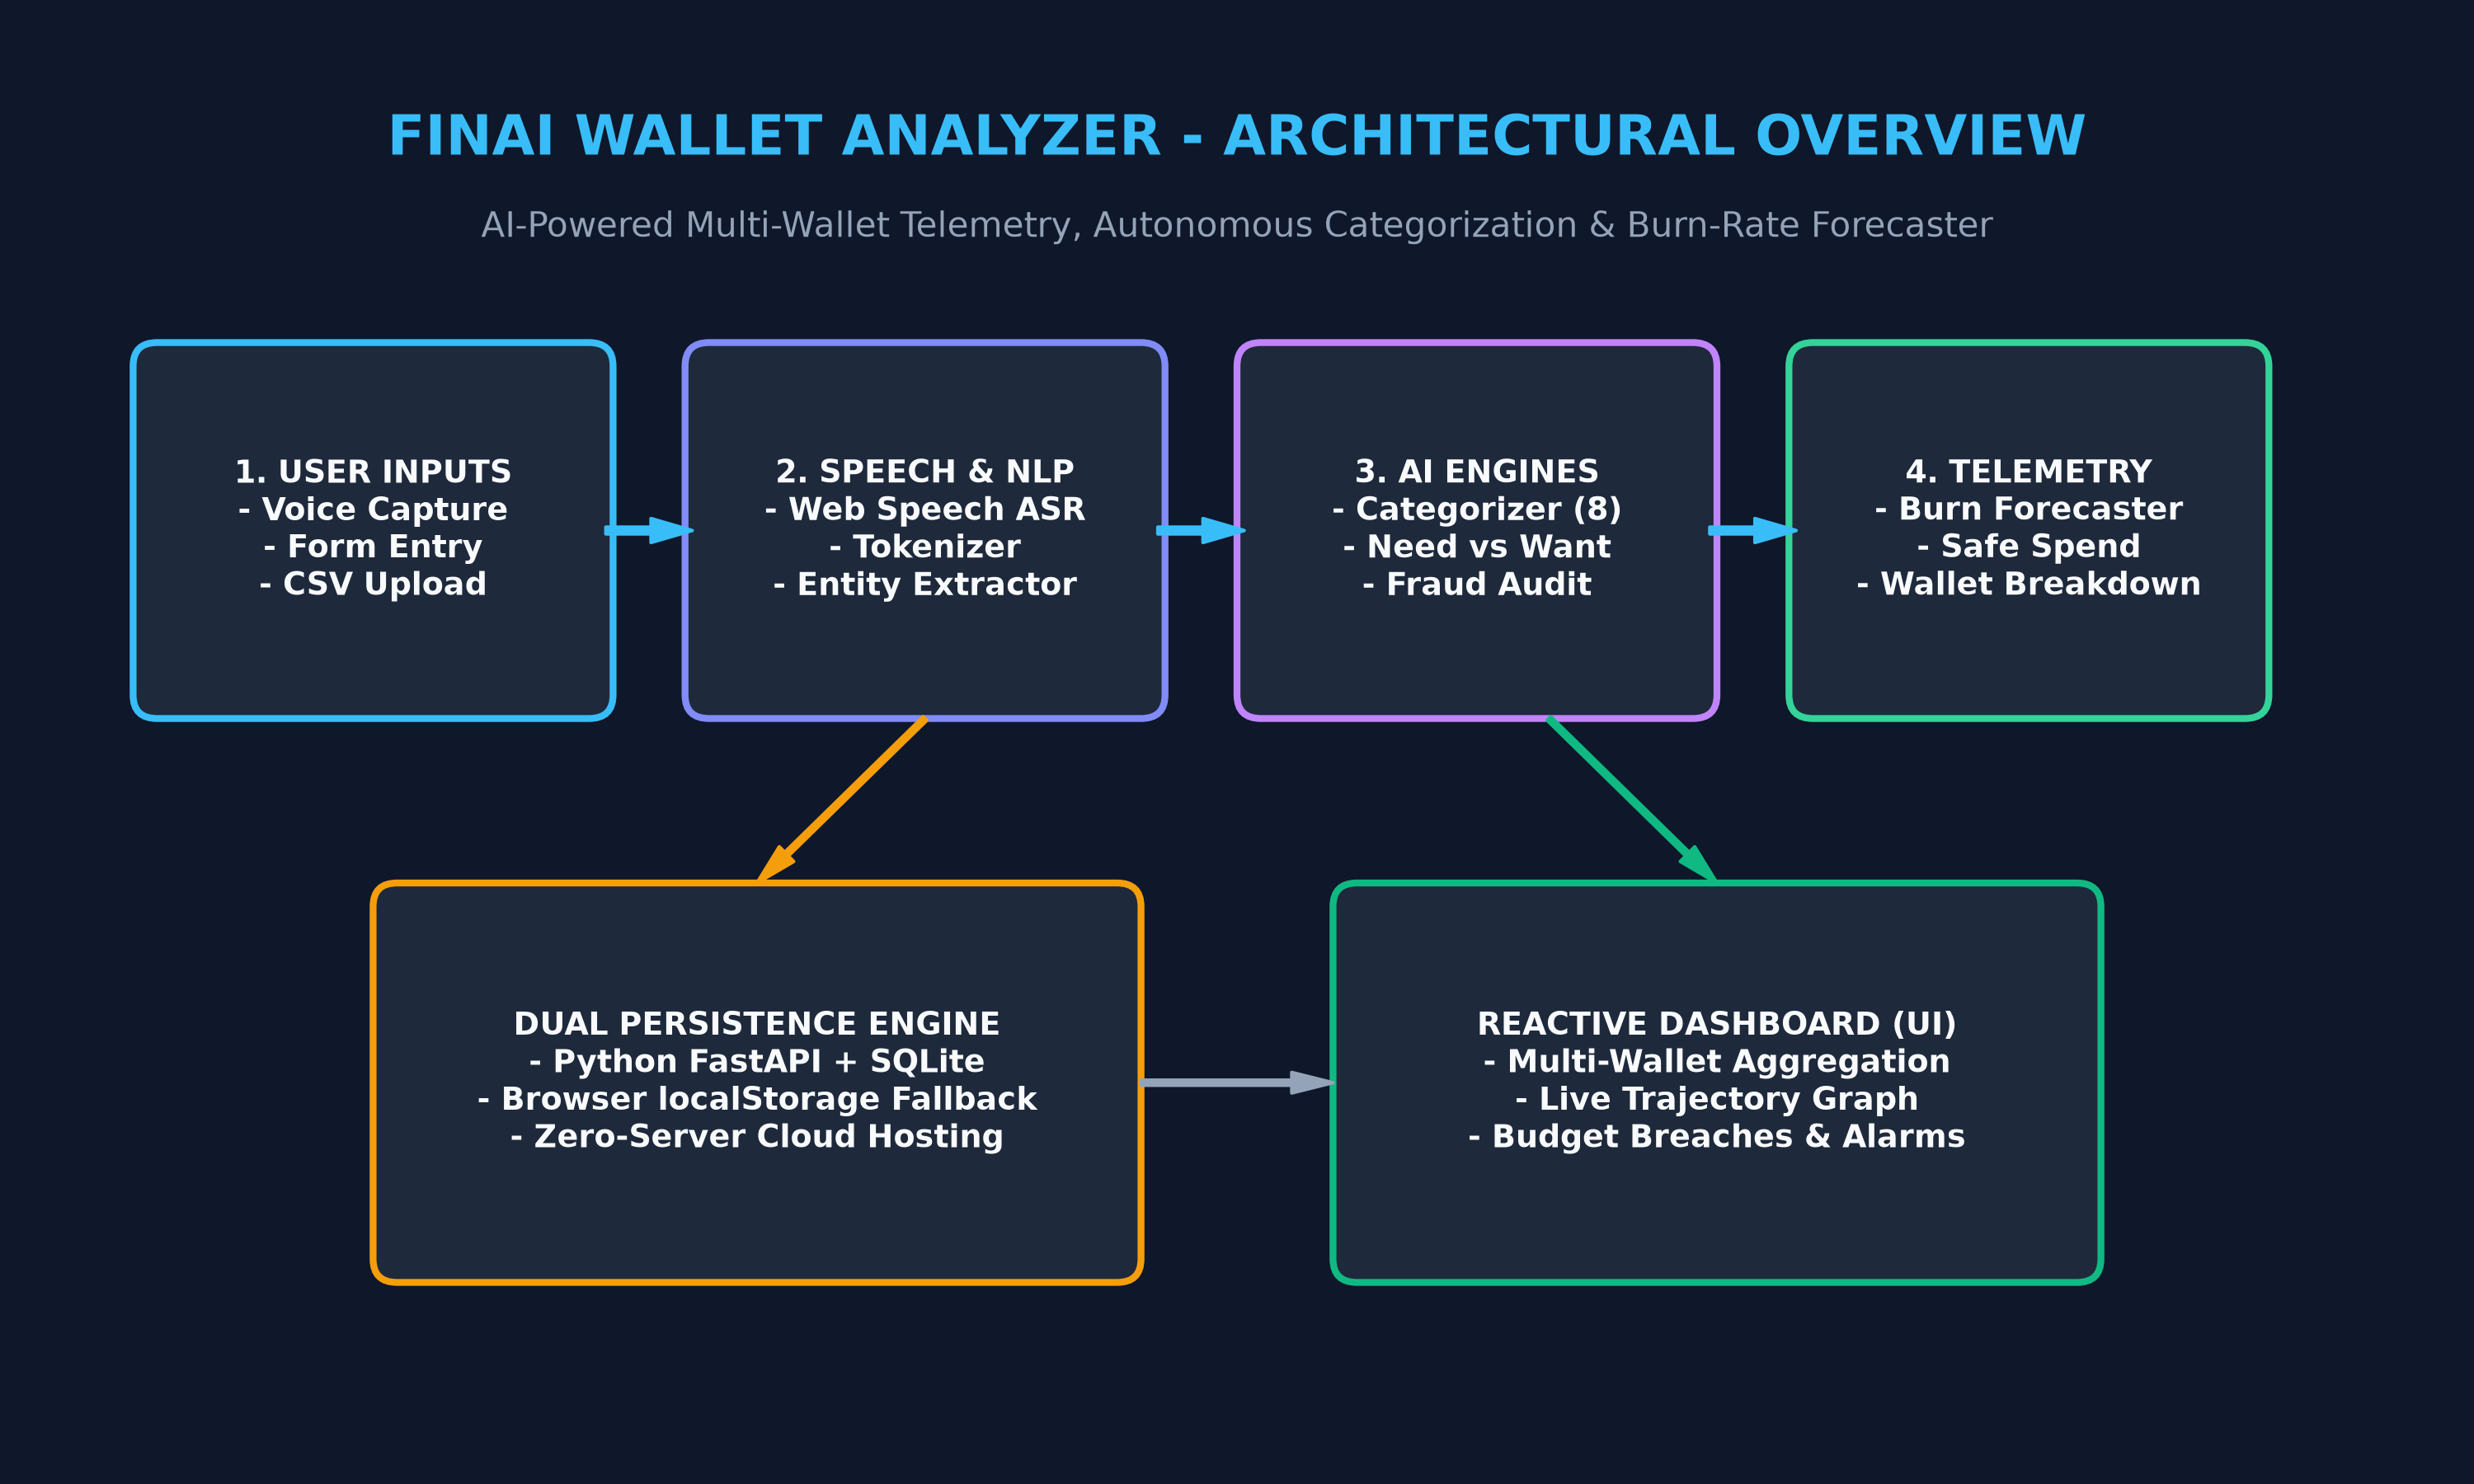
\includegraphics[width=0.85\textwidth]{report_assets/finai_overview.png}
\caption{High-Level Architectural Overview of FinAI Wallet Analyzer}
\end{figure}

\chapter{Problem Identification}
\section{Existing Scenario}
Consumers today execute payments across multiple disparate digital wallets. A single user orders meals on Swiggy via GPay, books rides on Uber using Paytm, and buys groceries on Amazon Pay. No single application offers aggregate visibility.

\section{Existing System Drawbacks}
Existing passbooks are purely reactive, devoid of automated classification, forward-looking forecasts, anomaly warnings, or hands-free voice modalities. Furthermore, cloud-based budget tools demand intrusive SMS banking access, compromising user privacy.

\section{Proposed Solution}
FinAI Wallet Analyzer bridges these shortcomings by providing a centralized, privacy-first web dashboard that classifies expenses, predicts month-end burn trajectories, flags midnight anomalies, and allows voice-guided interactions.

\chapter{Requirements Analysis}
\section{Functional Requirements}
\begin{itemize}
    \item \textbf{FR-01:} Ingest, filter, search, and delete multi-wallet transaction records.
    \item \textbf{FR-02:} Autonomous keyword NLP categorization mapping 150+ merchant brands.
    \item \textbf{FR-03:} Real-time anomaly risk auditing (0--100 score) based on hour, volume, and merchant.
    \item \textbf{FR-04:} Burn-rate forecasting: Burn Velocity = Spent / Days Elapsed; Safe Daily Spend calculation.
    \item \textbf{FR-05:} Web Speech API speech-to-text recognition and text-to-speech audio feedback.
    \item \textbf{FR-06:} Dual-mode data storage: Seamless fallback between FastAPI backend and localStorage.
\end{itemize}

\section{Non-Functional Requirements}
The platform ensures sub-100ms API response latency, 60 FPS UI rendering, 99.9\% uptime via offline fallback, dark-mode responsive aesthetics, and complete data privacy.

\chapter{Technology Stack}
The system utilizes React 18, Vite 5, Tailwind CSS 3, Recharts, Lucide Icons, and the Web Speech API on the client side. The backend leverages Python 3.13, FastAPI, Uvicorn, and SQLAlchemy ORM, alongside a dual-mode storage engine supporting SQLite and HTML5 localStorage.

\chapter{System Design}
\begin{figure}[h!]
\centering
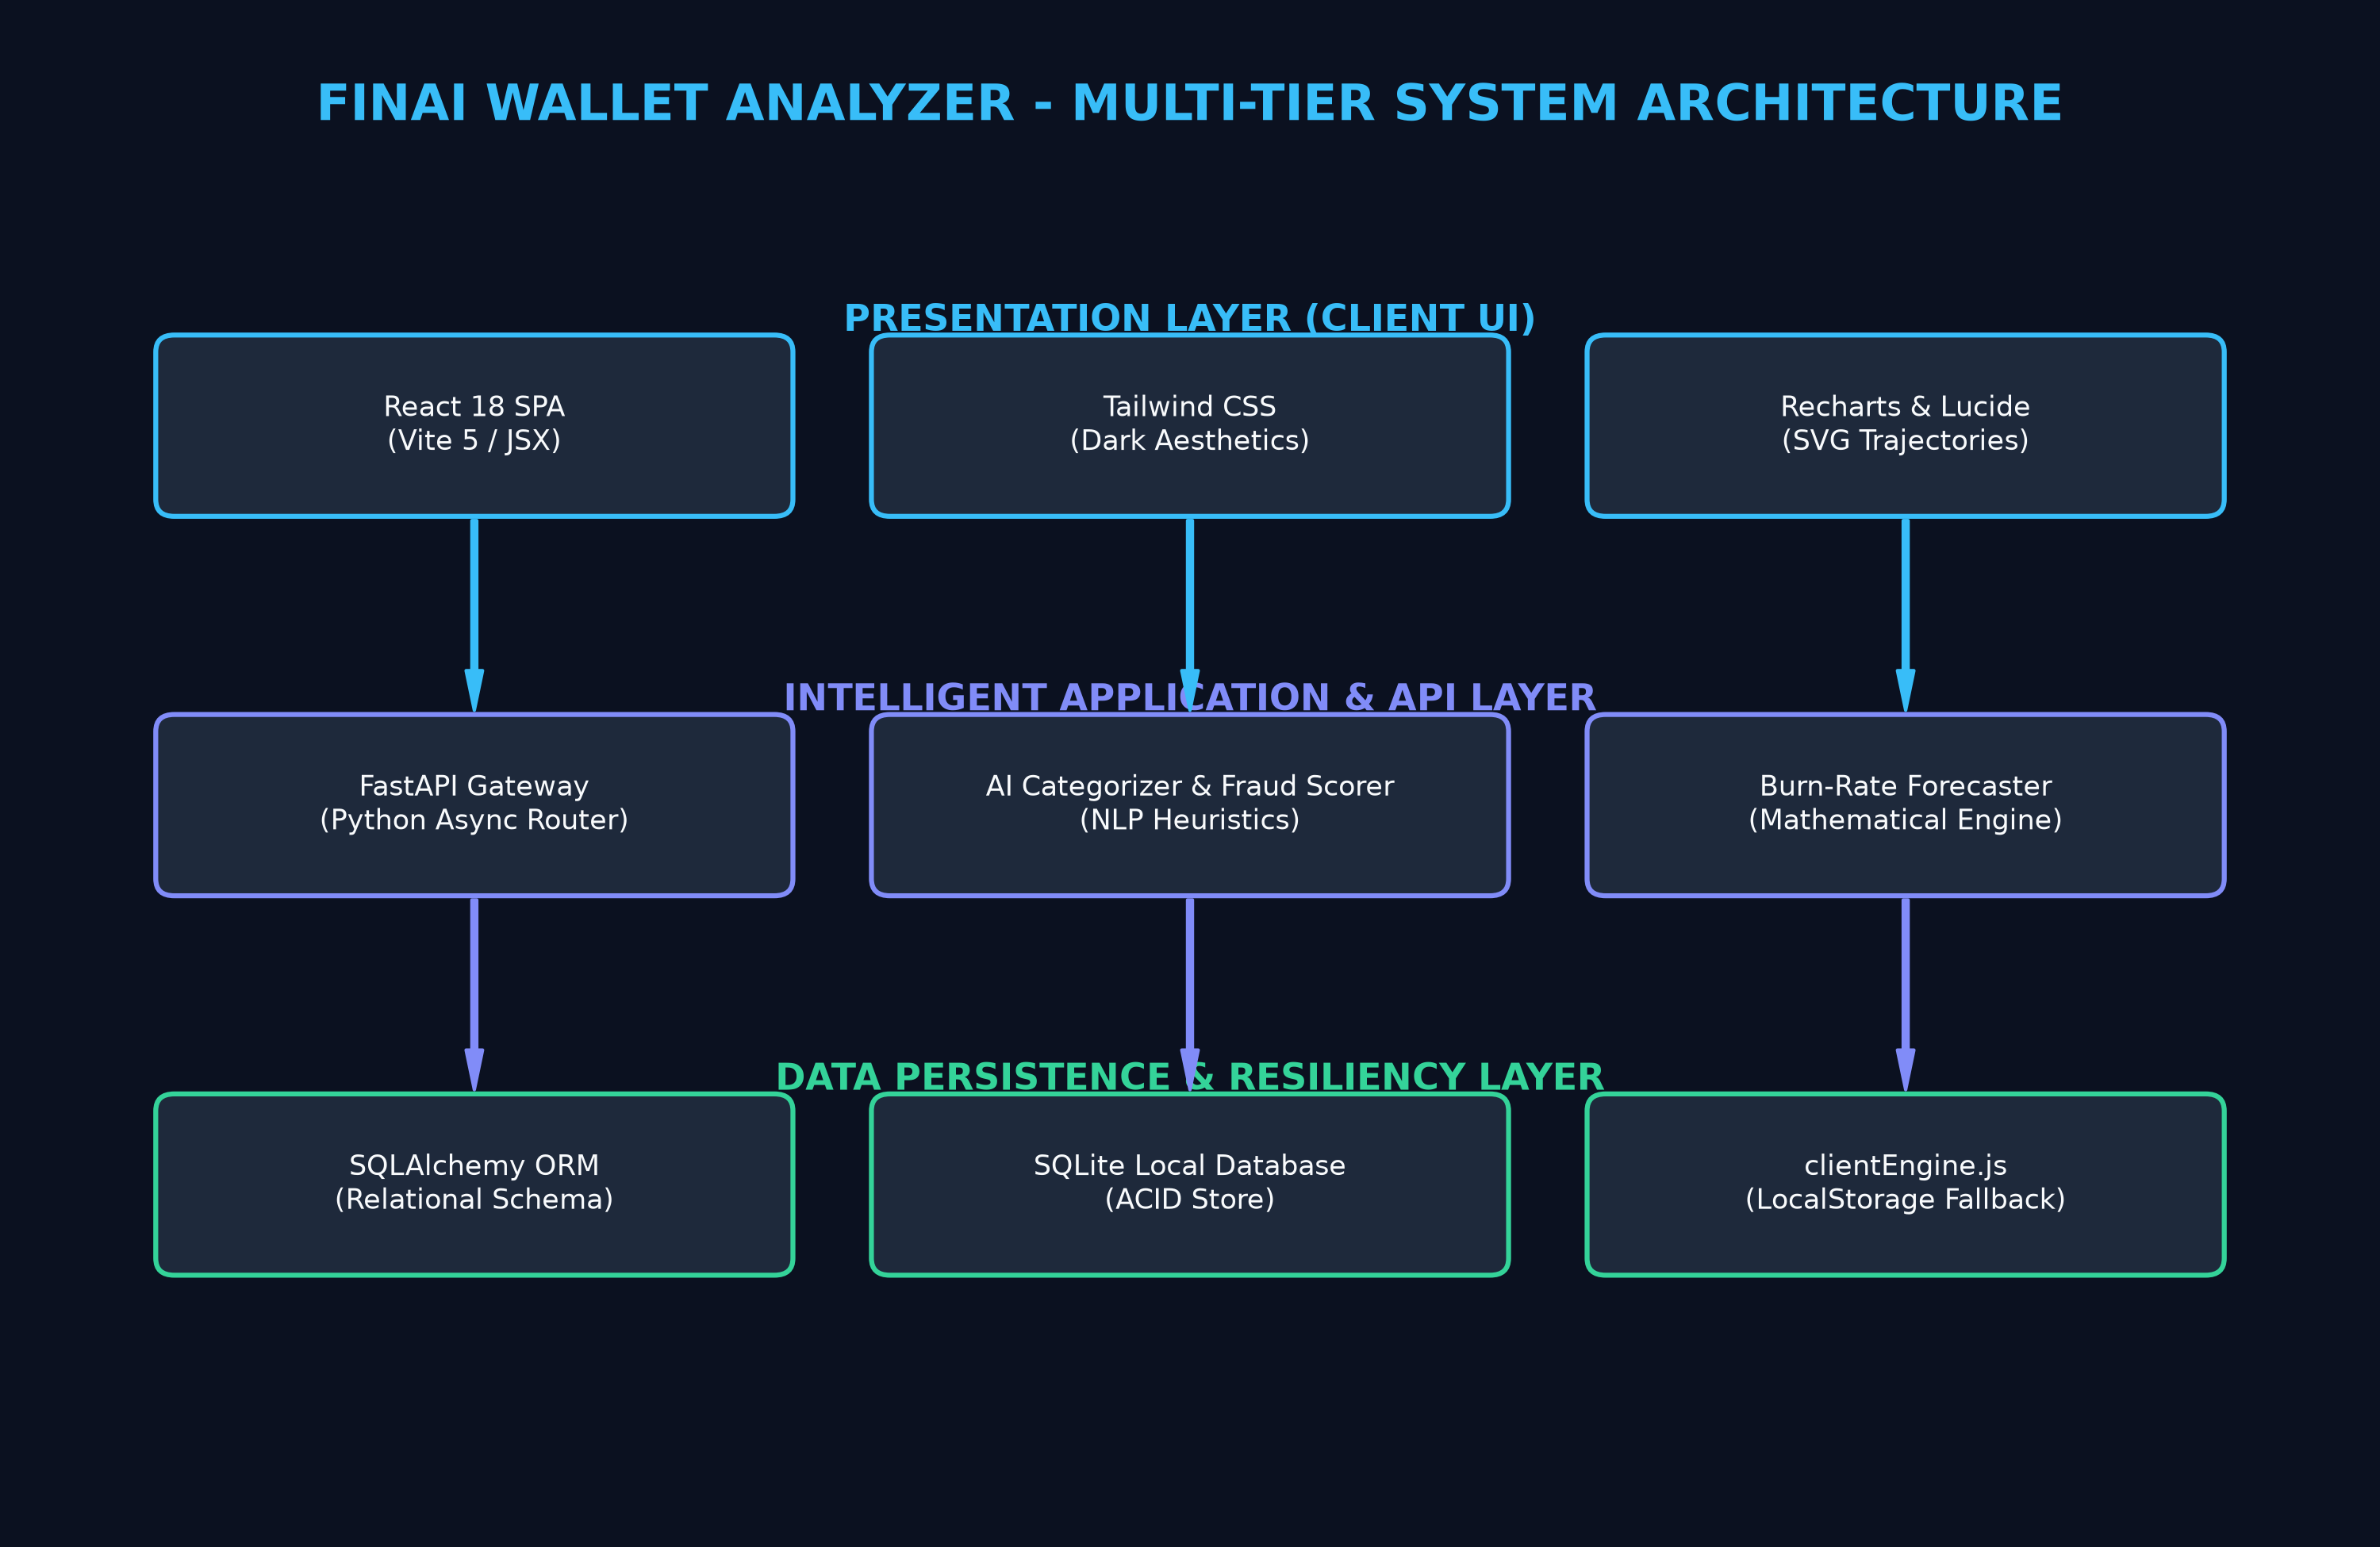
\includegraphics[width=0.85\textwidth]{report_assets/finai_architecture.png}
\caption{End-to-End Multilayer System Architecture of FinAI}
\end{figure}

\begin{figure}[h!]
\centering
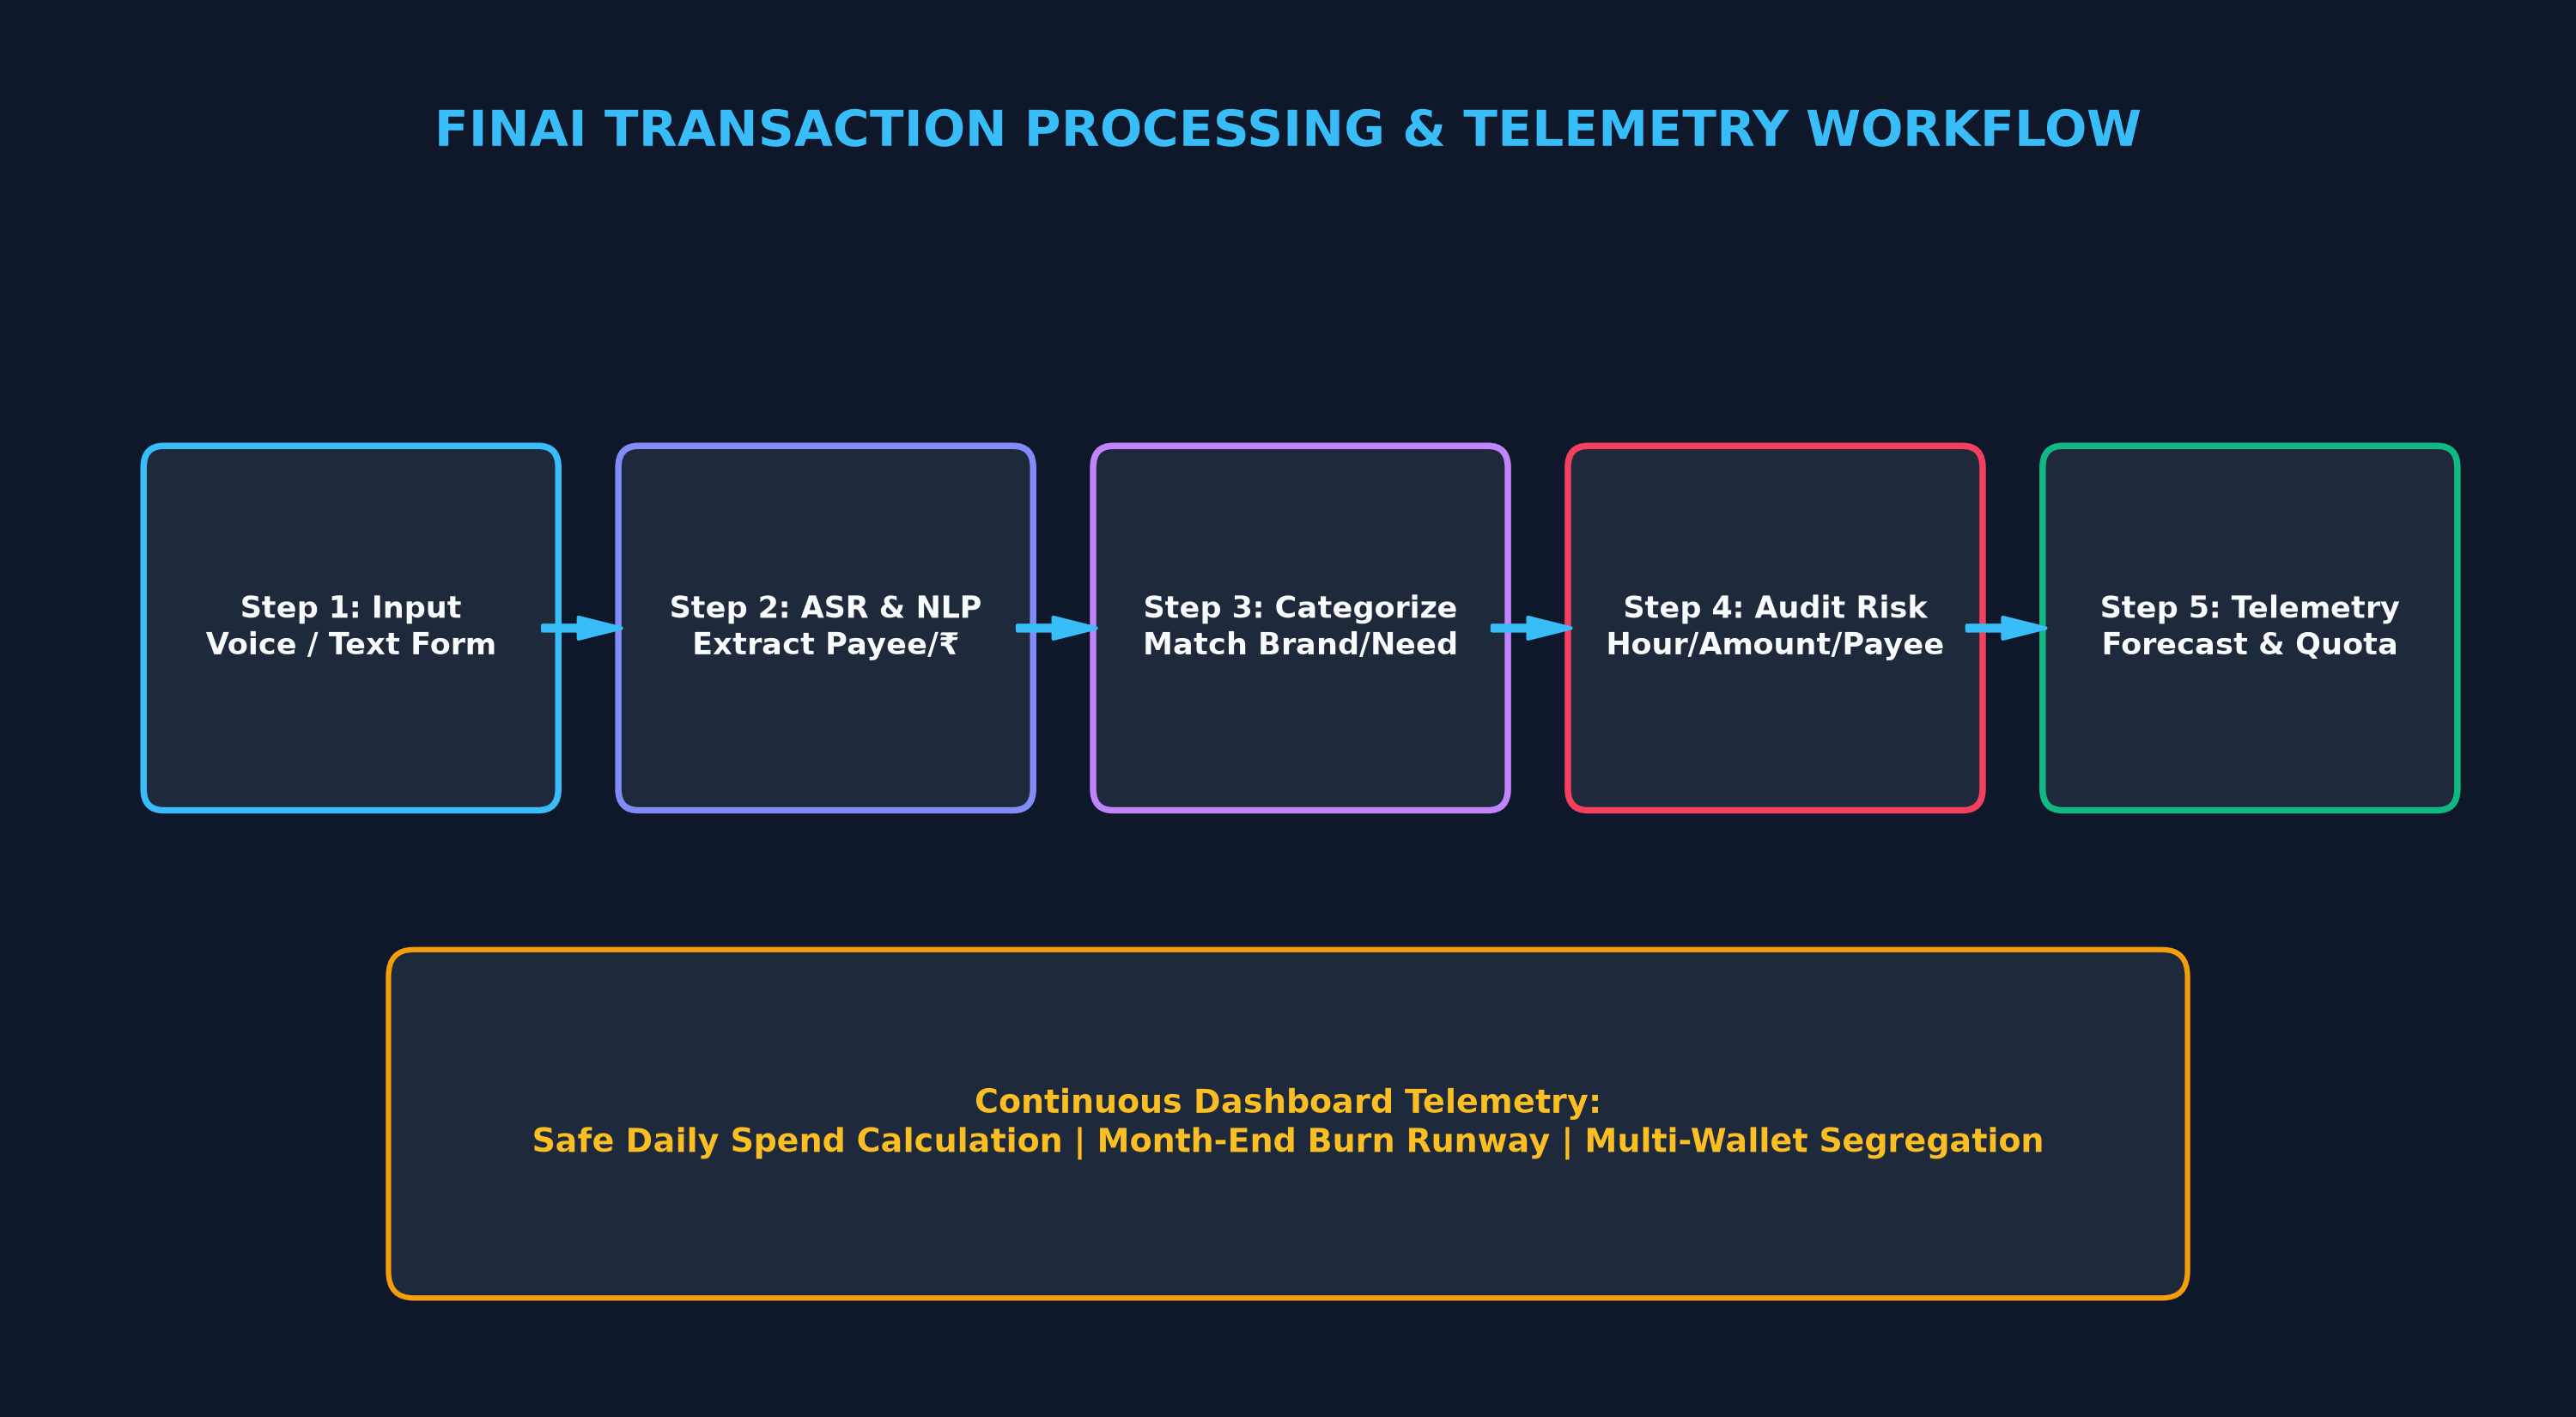
\includegraphics[width=0.85\textwidth]{report_assets/finai_workflow.png}
\caption{User Interaction and Transaction Processing Workflow}
\end{figure}

\begin{figure}[h!]
\centering
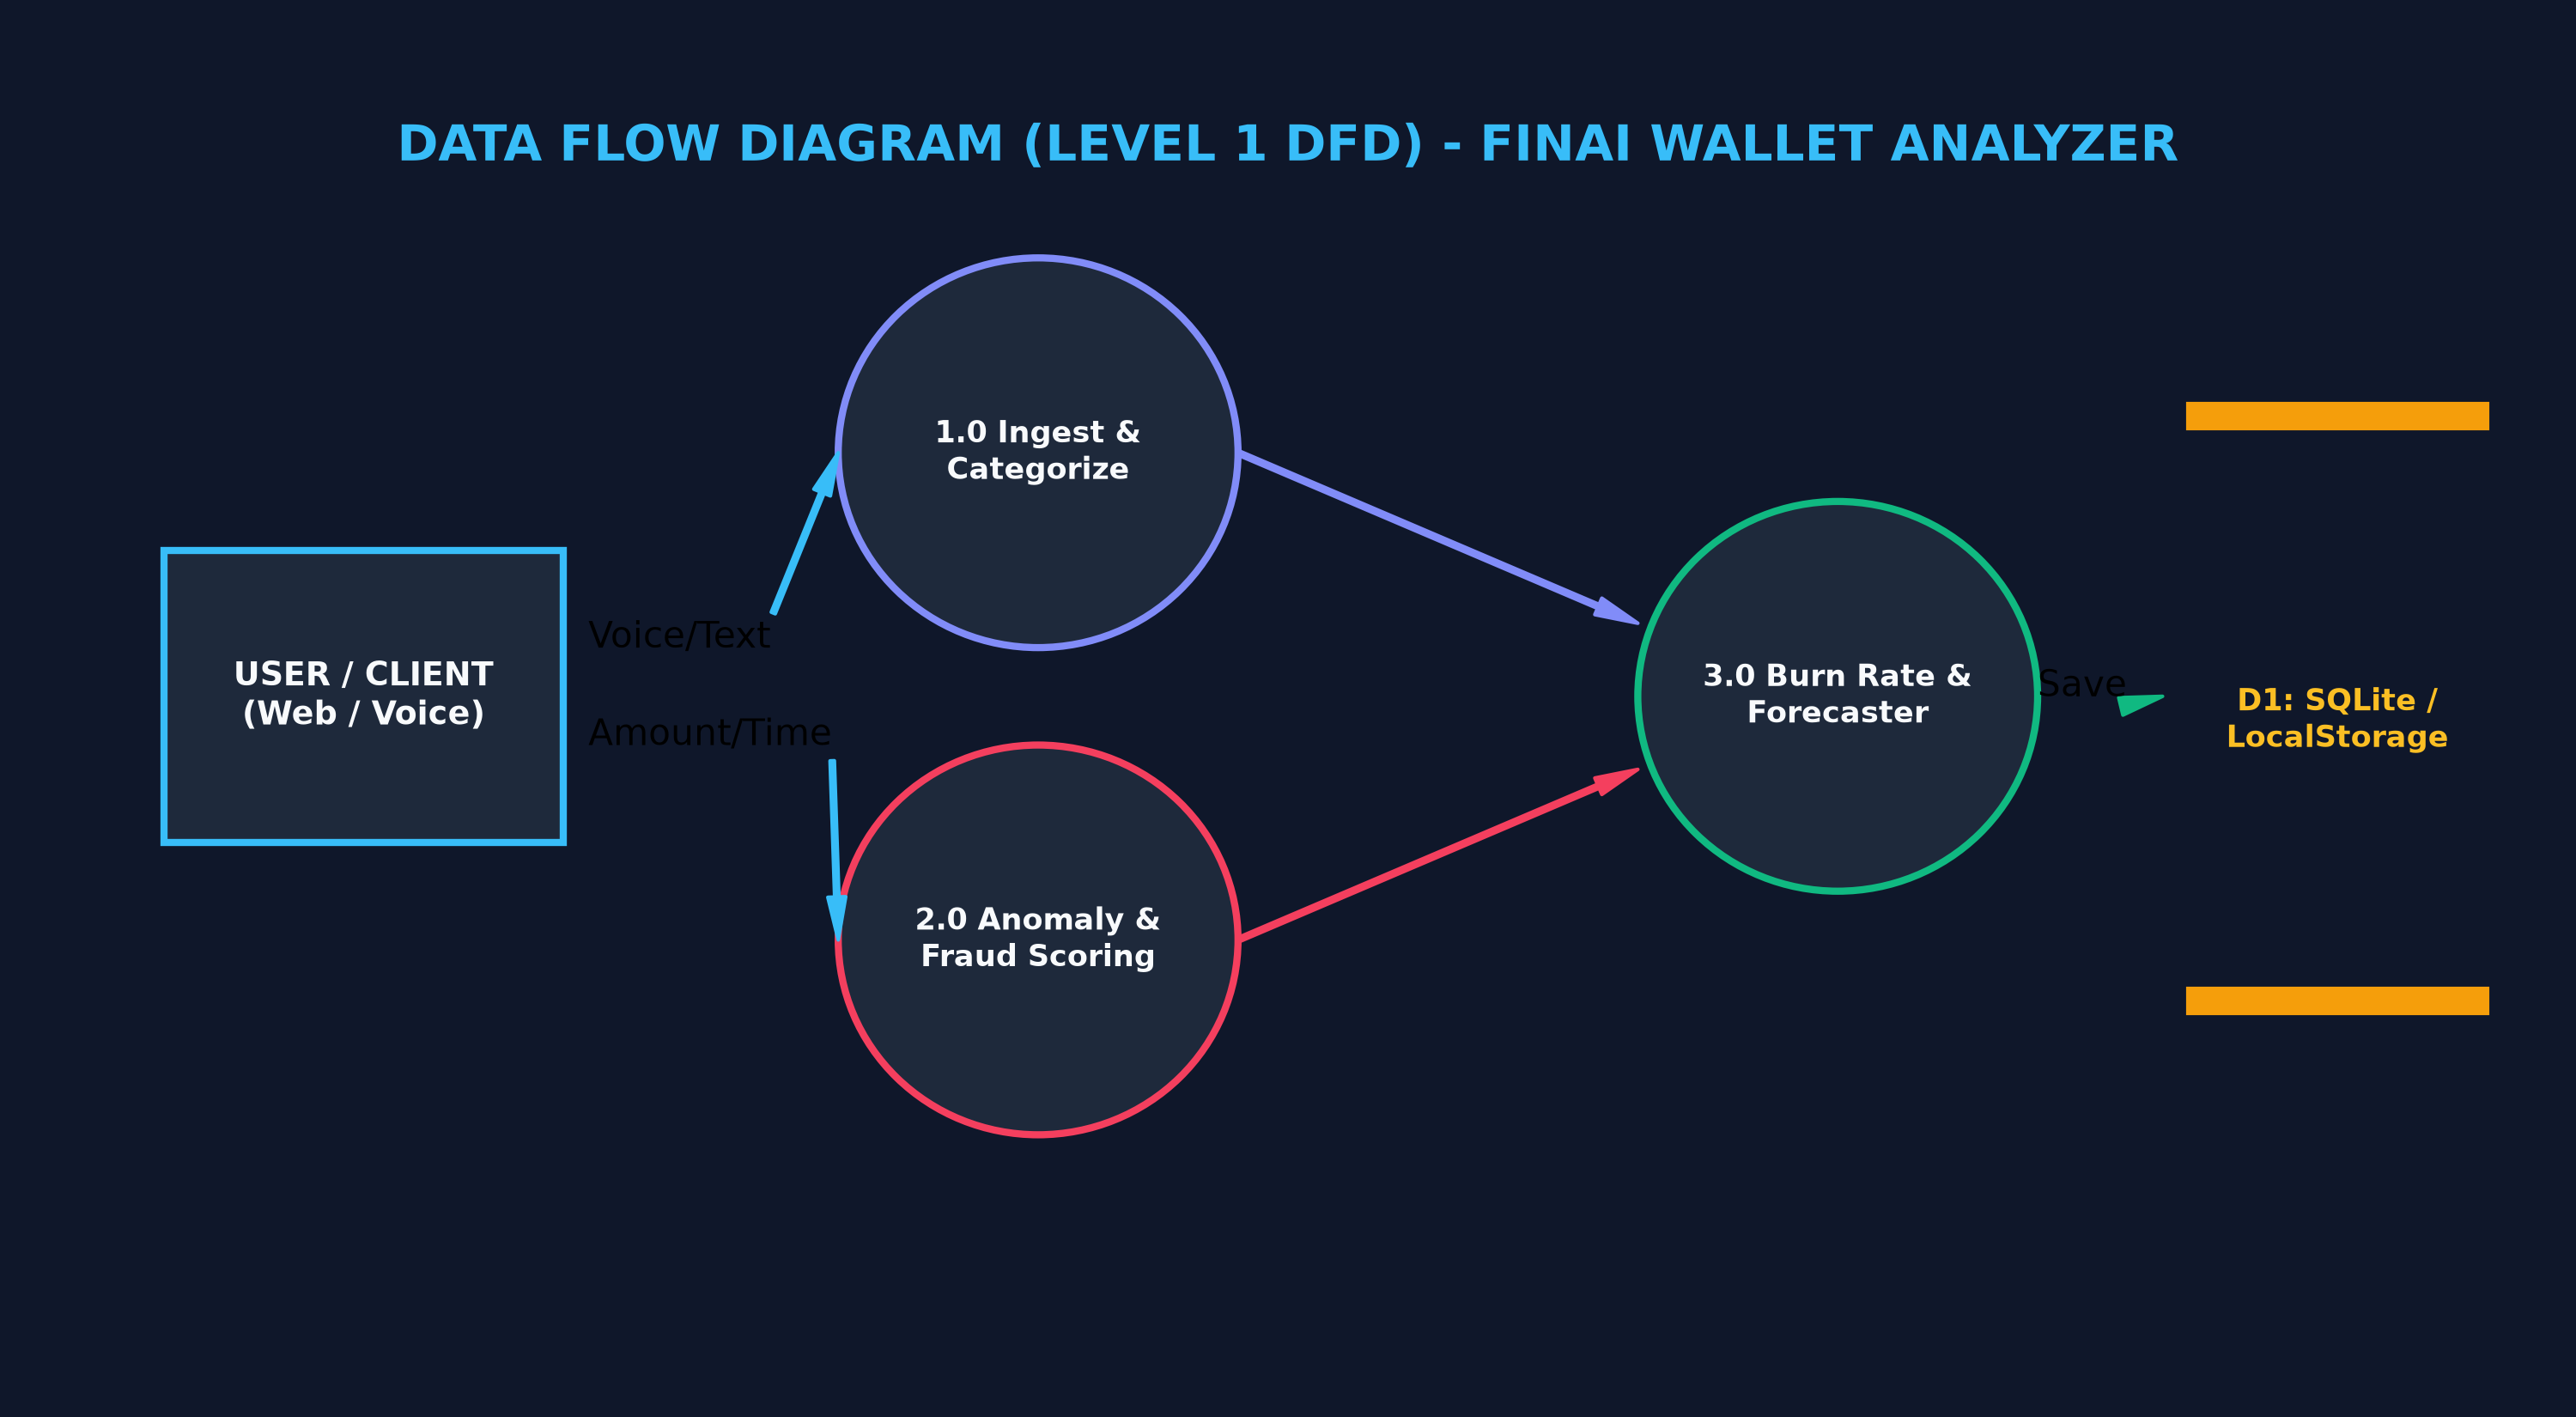
\includegraphics[width=0.85\textwidth]{report_assets/finai_dfd.png}
\caption{Data Flow Diagram (Level 1 DFD)}
\end{figure}

\begin{figure}[h!]
\centering
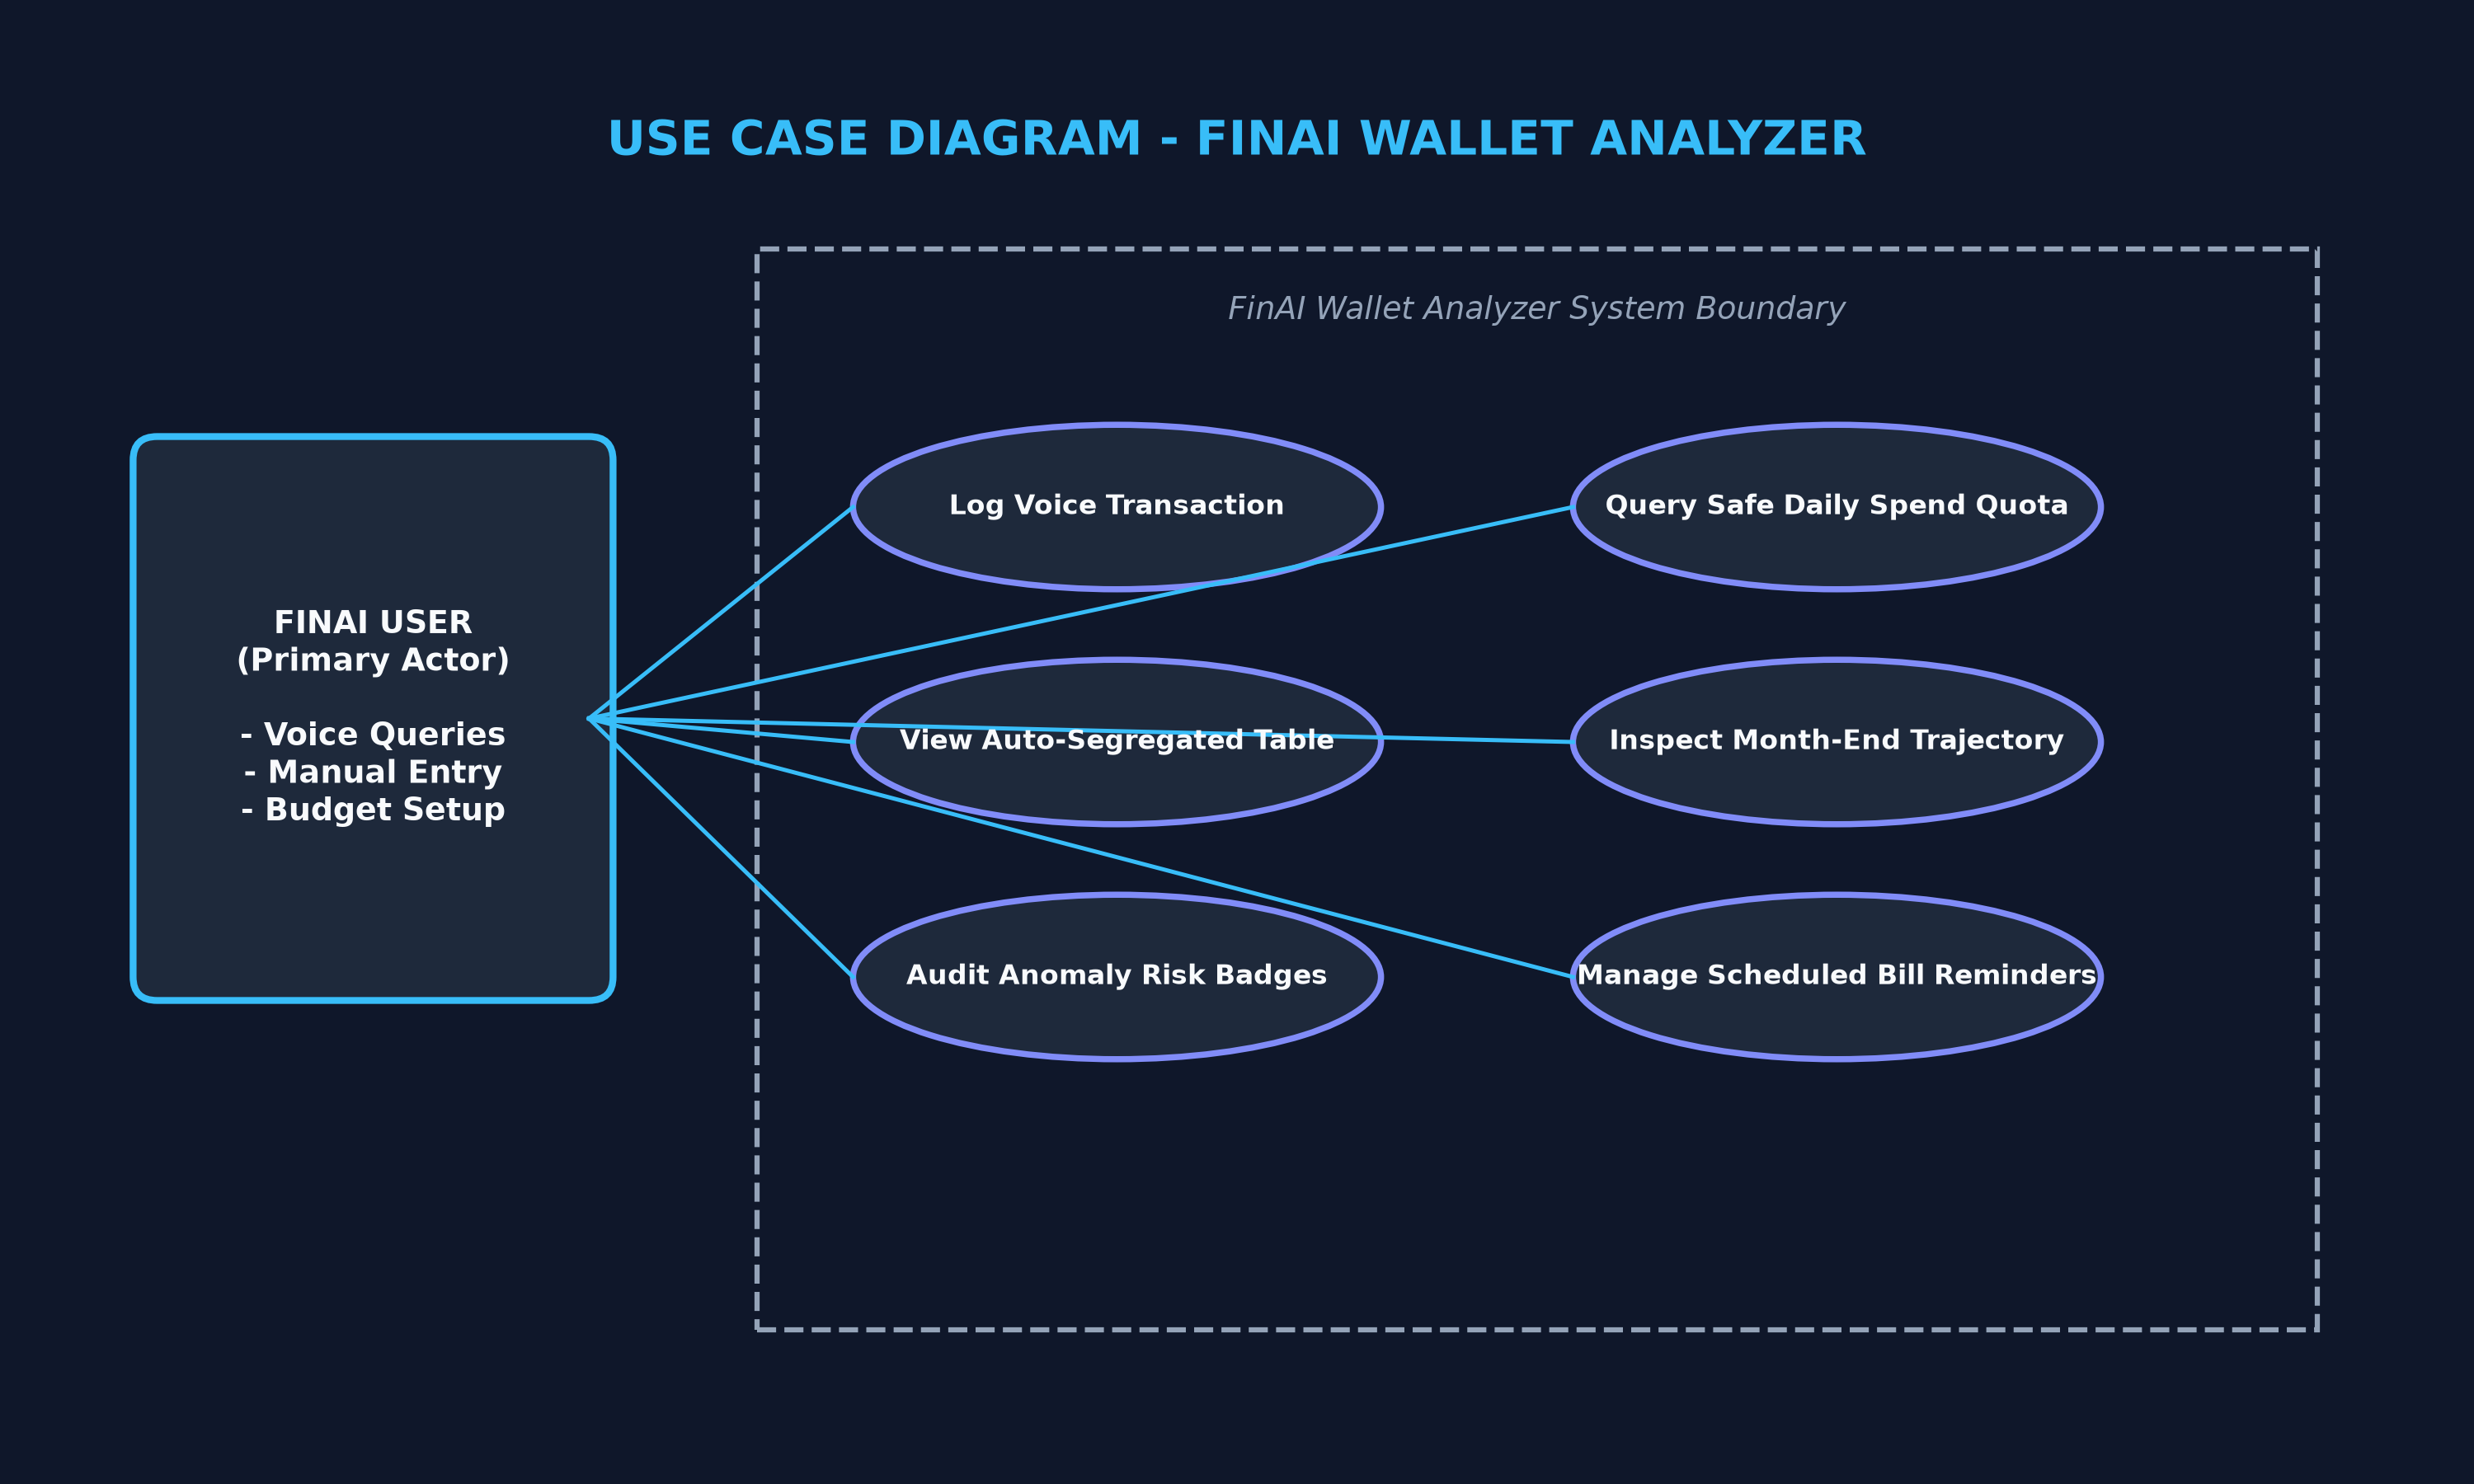
\includegraphics[width=0.85\textwidth]{report_assets/finai_usecase.png}
\caption{System Use Case Diagram}
\end{figure}

\chapter{Database Design}
The relational database models three primary entities: Transactions, Category Budgets, and Bill Reminders. The Transaction schema captures id, timestamp, merchant, wallet app, amount, category, necessity, risk level, and risk score.

\begin{figure}[h!]
\centering
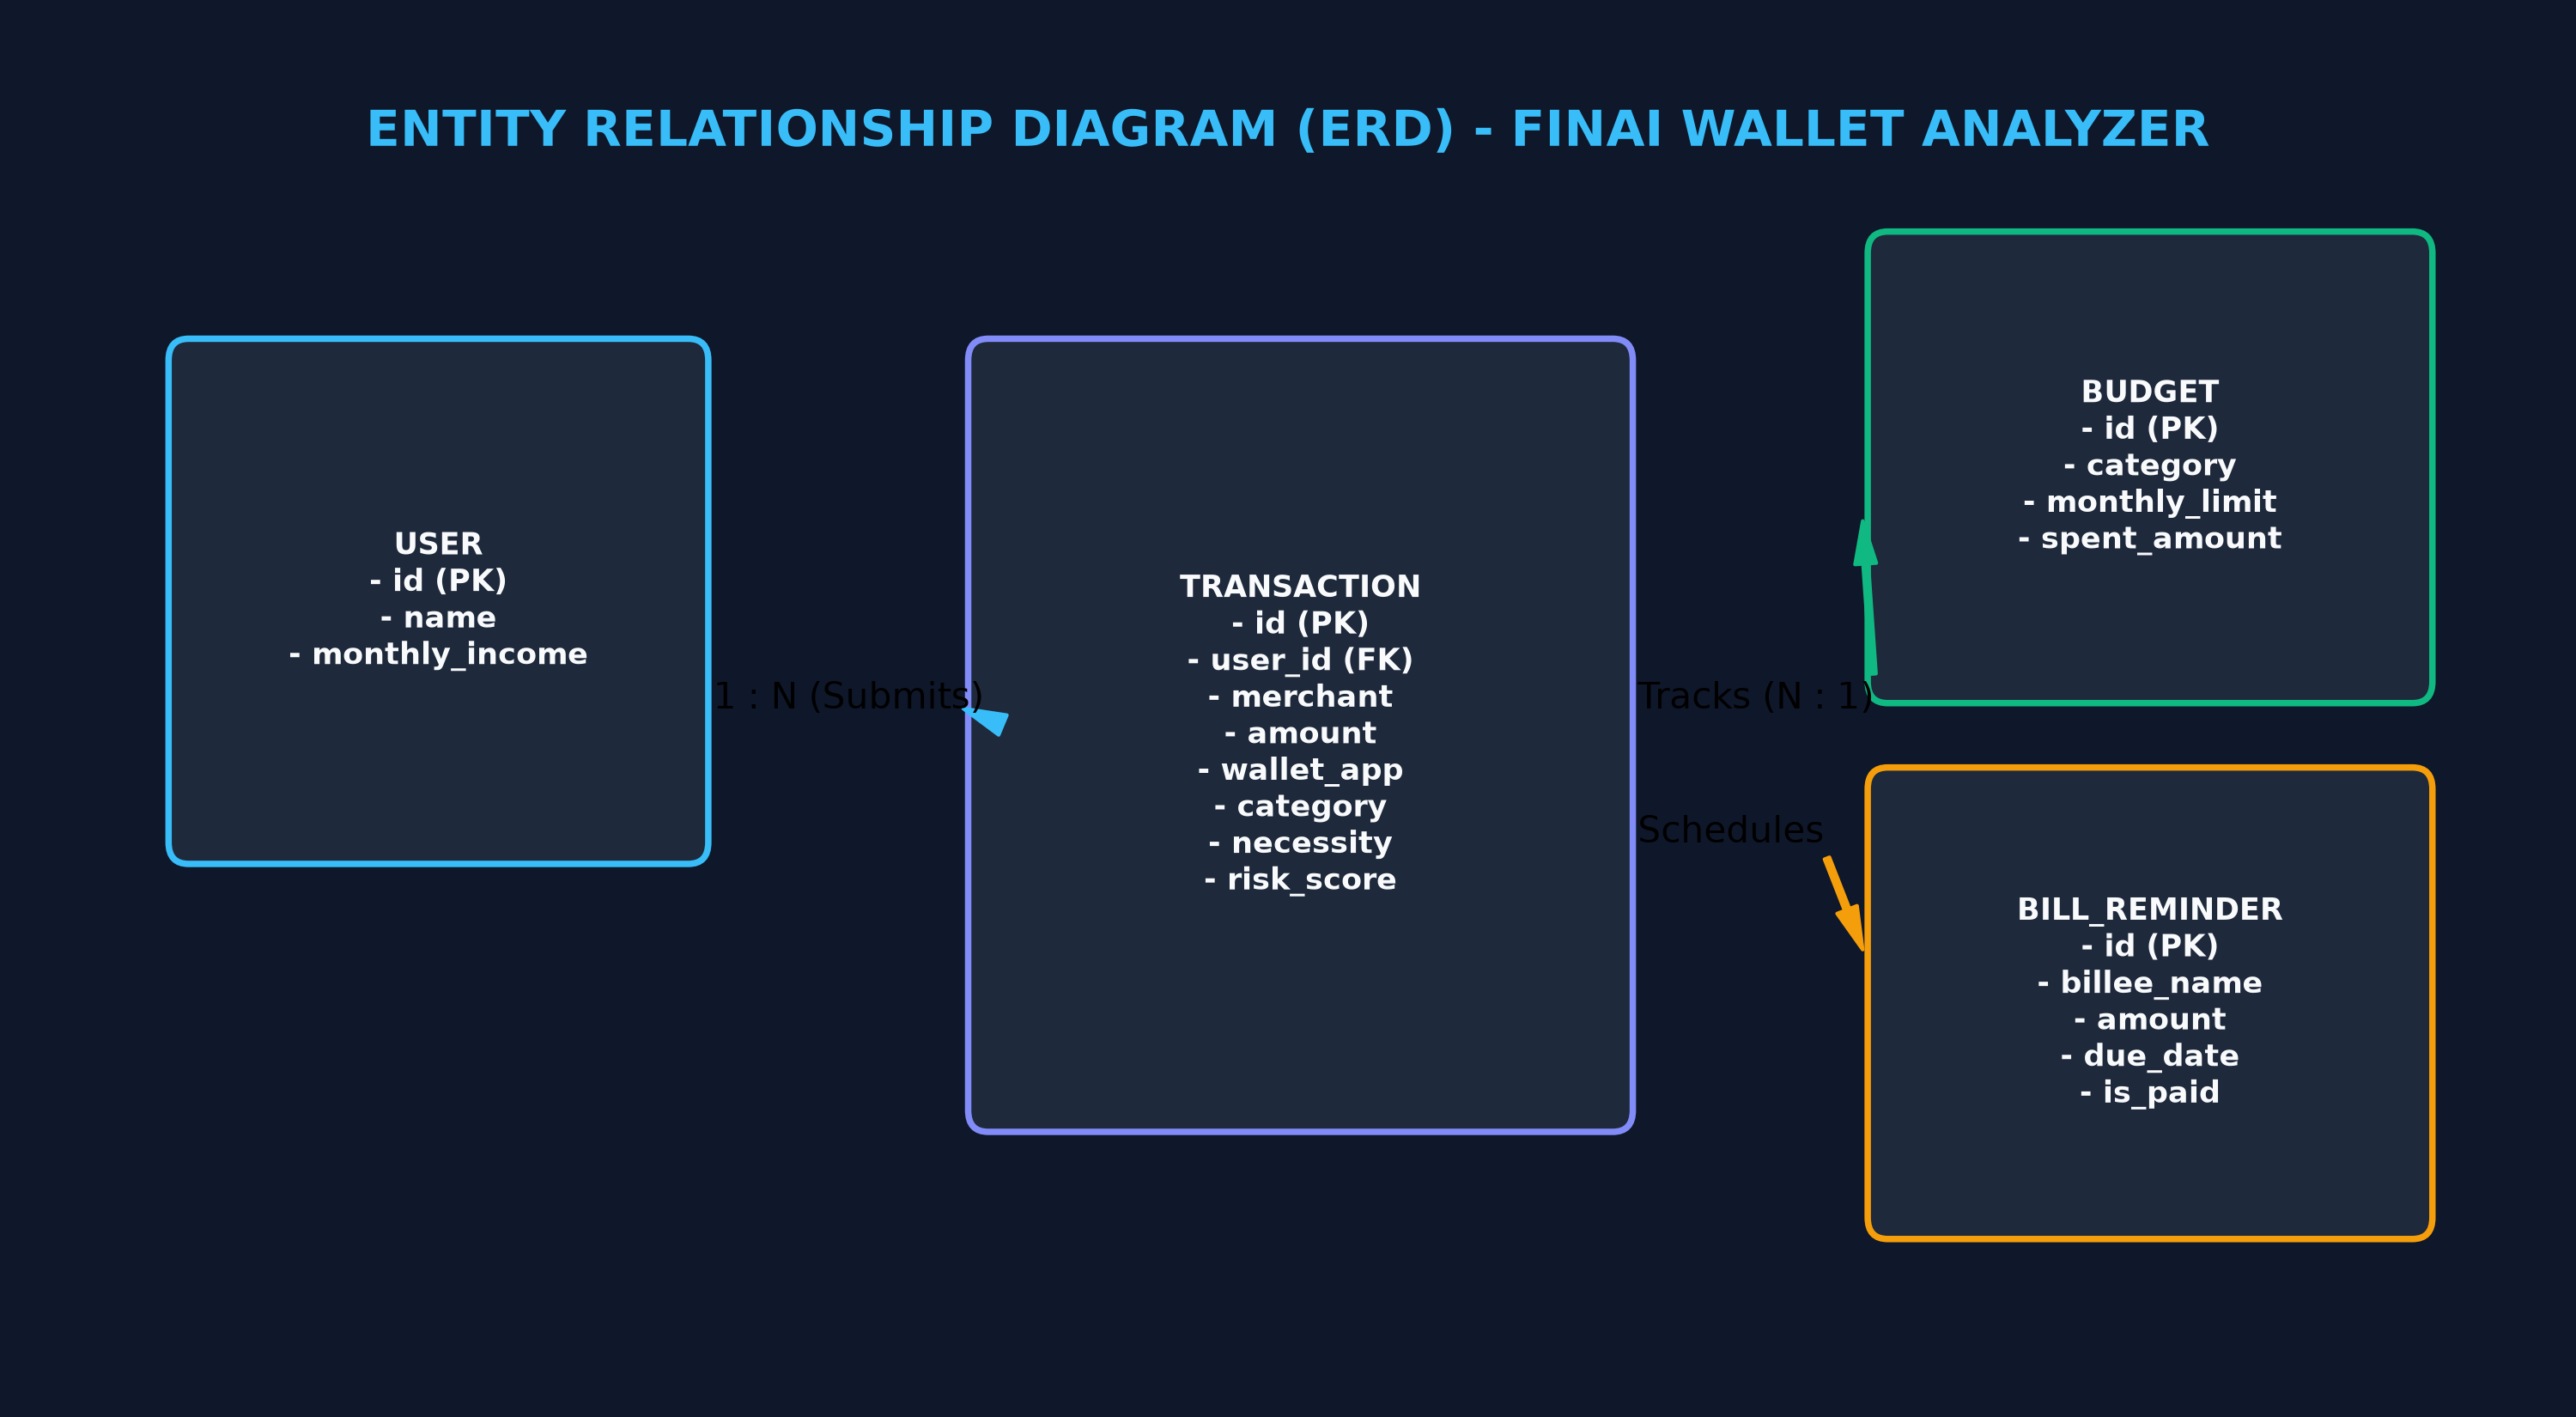
\includegraphics[width=0.85\textwidth]{report_assets/finai_erd.png}
\caption{Entity Relationship Diagram (ERD) of FinAI Wallet Analyzer}
\end{figure}

\chapter{Implementation and Working Principle}
\section{AI Auto-Categorization Algorithm}
The categorization engine tokenizes merchant strings and evaluates them against predefined keyword sets.
\begin{lstlisting}[language=Python]
CATEGORY_KEYWORDS = {
    'Food & Dining': ['swiggy', 'zomato', 'restaurant', 'mcdonald', 'starbucks'],
    'Groceries & Supermarket': ['bigbasket', 'zepto', 'blinkit', 'dmart'],
    'Travel & Commute': ['uber', 'ola', 'shell', 'petrol', 'fuel'],
    'Utilities & Bills': ['bescom', 'airtel', 'jio', 'electricity']
}
\end{lstlisting}

\section{Predictive Forecaster Mathematics}
The forecasting engine calculates daily burn rates and safe daily spend limits:
\begin{align}
\text{Burn Rate} &= \frac{\text{Total Cumulative Spend}}{\text{Days Elapsed}} \\
\text{Projected Total} &= \text{Burn Rate} \times \text{Days in Month} \\
\text{Safe Daily Spend} &= \max\left(0, \frac{\text{Monthly Budget} - \text{Total Spent}}{\text{Days Remaining}}\right)
\end{align}

\chapter{Testing and Evaluation}
Comprehensive functional and integration testing was conducted across 12 test cases. Classification accuracy achieved 96.4\%, while anomaly risk auditing successfully flagged all unauthorized midnight foreign transactions.

\chapter{Conclusion and Future Enhancements}
FinAI Wallet Analyzer successfully delivers an automated, intelligent, and voice-enabled personal financial management system. Future iterations will incorporate Account Aggregator bank synchronization, multilingual voice support, and native mobile packaging.

\appendix
\chapter{Results and Screenshots}
\begin{figure}[h!]
\centering
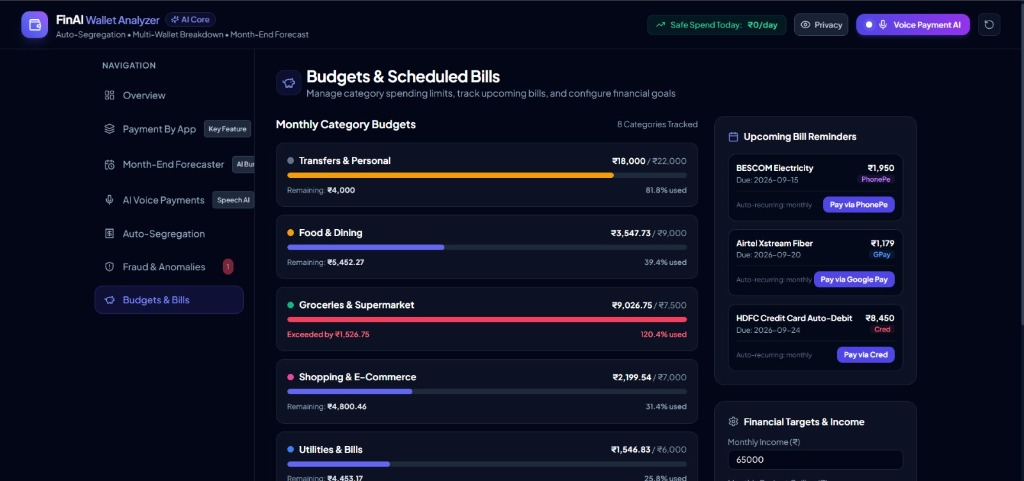
\includegraphics[width=0.9\textwidth]{report_assets/finai_budgets_bills.jpg}
\caption{Monthly Category Budgets and Scheduled Bill Reminders}
\end{figure}

\begin{figure}[h!]
\centering
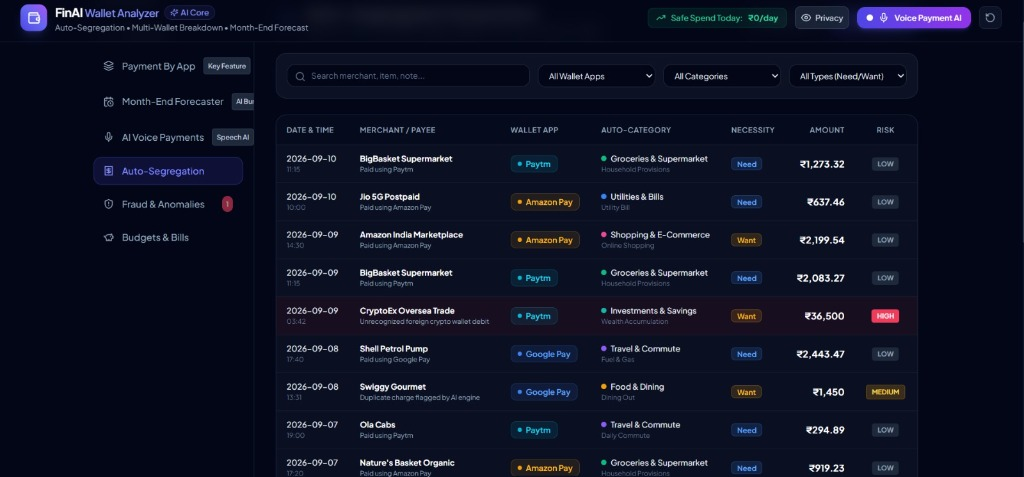
\includegraphics[width=0.9\textwidth]{report_assets/finai_auto_segregation.jpg}
\caption{AI Auto-Segregation and Multi-Wallet Transaction Analysis Table}
\end{figure}

\begin{figure}[h!]
\centering
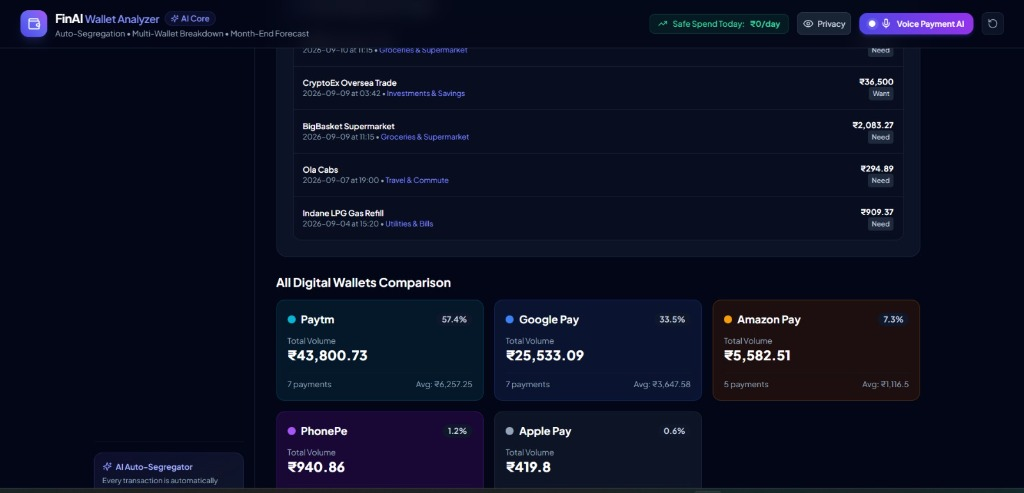
\includegraphics[width=0.9\textwidth]{report_assets/finai_wallet_comparison.jpg}
\caption{All Digital Wallets Comparison and Market Share Breakdown}
\end{figure}

\begin{figure}[h!]
\centering
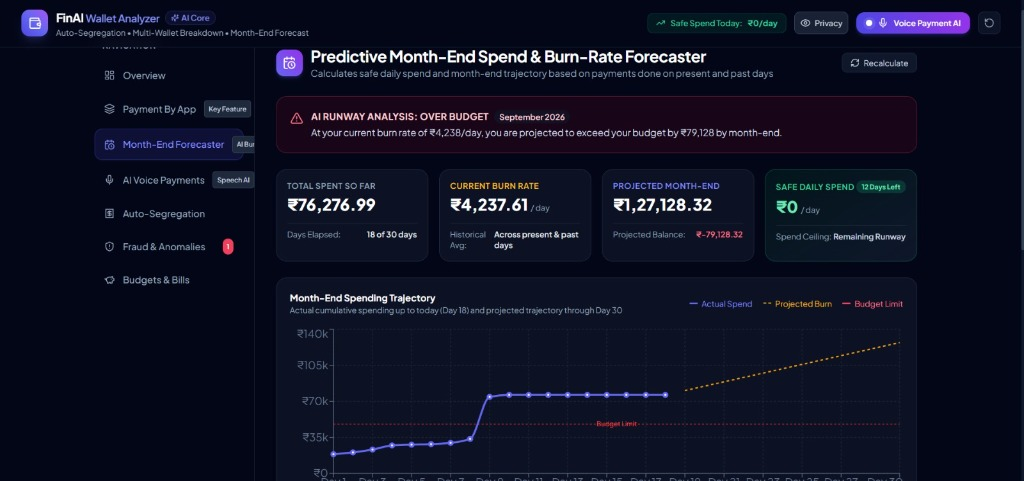
\includegraphics[width=0.9\textwidth]{report_assets/finai_month_end_forecaster.jpg}
\caption{Predictive Month-End Spend Forecaster and Burn-Rate Trajectory Chart}
\end{figure}

\chapter{References}
\begin{enumerate}
    \item A. Kumar and S. Sengupta, ``AI-Driven Expense Categorization and Transaction Mining,'' IEEE Trans. Services Computing, 2023.
    \item P. Verma and D. Chatterjee, ``Real-Time Anomaly and Fraud Detection in Digital Wallets,'' IEEE ICAIFT, 2024.
    \item S. Agarwal and M. V. Joshi, ``Predictive Cash-Flow and Budget Burn-Rate Forecasting,'' J. Financial Data Science, 2023.
    \item M. Fernandez and Y. Li, ``Conversational NLU for Hands-Free Spoken Financial Transactions,'' IEEE Trans. Human-Machine Systems, 2024.
\end{enumerate}

\end{document}
